\PassOptionsToPackage{cmyk,table}{xcolor}
% pbalance back in for camera-ready: below one column of text it aborts pdflatex on infinite glue.
\documentclass[conference]{iaria}
\pdfoutput=1

% BEWARE: iaria.cls requires this TeX stack: pdflatex/biblatex/biber!

% !TeX spellcheck = en-US
% !TeX encoding = utf8
% !TeX program = pdflatex
% !BIB program = biblatex / biber

% --- Language & quotation marks ---
\usepackage[babel=true,english=american]{csquotes}
\usepackage[english]{babel} % en-US

% --- Additional packages for tables/units ---
\usepackage{booktabs}
\usepackage{siunitx}
\usepackage[nohyperlinks]{acronym}

\acrodef{API}{application programming interface}
\acrodef{CPU}{central processing unit}
\acrodef{CSV}{comma-separated values}
\acrodef{IQR}{interquartile range}
\acrodef{LAN}{local area network}
\acrodef{VM}{virtual machine}
\acrodef{VMM}{virtual machine monitor}
\acrodef{WASM}{WebAssembly}

% --- Bibliography (bib file; style/backend come from iaria.cls) ---
\addbibresource{references.bib}

% floatrow sets \textwidth to \columnwidth inside a float, and a float can trigger \output there.
\makeatletter
\AtBeginDocument{\edef\paper@textwidth{\the\textwidth}}
\pretocmd{\@outputdblcol}{\textwidth\paper@textwidth\relax}{}{\PackageError{main}{patch failed}{}}
\makeatother

% --- Metadata ---
\hypersetup{
  pdftitle={Migration Without Memory: Session Handover Across the Browser-to-microVM Isolation Boundary},
  pdfauthor={Jane Schönfeld, Nils Mohr, Malte Prieß}
}

\title{Migration Without Memory:\\ Session Handover Across the Browser-to-microVM Isolation Boundary}

\author{
    \IEEEauthorblockN{
        Jane Schönfeld\IEEEauthorrefmark{1},
        Dr. Nils Mohr\IEEEauthorrefmark{2},
        Prof. Dr. Malte Prieß\IEEEauthorrefmark{1}
    }
    \IEEEauthorblockA{
        \IEEEauthorrefmark{1}Department of Computer Science and Electrical Engineering,
        University of Applied Sciences (HAW) Kiel, Germany\\
        e-mail: \texttt{jane.schoenfeld@stu.haw-kiel.de}, \texttt{malte.priess@haw-kiel.de}
    }
    \IEEEauthorblockA{
        \IEEEauthorrefmark{2}CODEANKER GmbH, Flensburg, Germany\\
        e-mail: \texttt{nils.mohr@codeanker.de}
    }
}

\hyphenation{WebContainers Web-Assem-bly}

\begin{document}

\maketitle
\thispagestyle{plain}
\pagestyle{plain}

\begin{abstract}
A development environment in WebContainers runs on the WebAssembly runtime inside the browser tab. Hence, it starts quickly and uses the capacity of the client. If a session runs out of resources, it may have to be handed over to a microVM on the server. The migration of a virtual machine transfers memory pages, but the WebContainers application programming interface documents an export for the filesystem and not for the memory. Without a memory image, three parts of migration theory still apply, the split into cold and live migration, the downtime and the total migration time. Cold migration, pre-copy, post-copy and hybrid migration all have a counterpart at the filesystem level, each with its own condition. Pre-copy requires an anticipated handover, post-copy requires the browser tab to stay open until all files have been fetched, and hybrid migration requires both. Pre-copy and cold migration are measured as the interruption time of a small heartbeat process, from its stop in the browser to its restart in a microVM on the hosted service E2B. On the largest of four project sizes, the full copy (cold migration) sends the whole project after the stop and has a median interruption time of \SI{8.74}{\second}. Pre-copy sends the project once to a target created before the stop, which lowers the median interruption time to \SI{1.69}{\second}. However, pre-copy takes \SI{1.16}{\second} longer in total than the full copy. Without anticipation, the full copy is compared with manifest-based transfer, which sends the project without its dependencies and installs them on the target. For the four projects on E2B, manifest-based transfer is faster from a size between \SI{4.62}{\mega\byte} and \SI{13.93}{\mega\byte}. This size may also depend on their packages, on the uplink of the client and on the registry link of the target.
\end{abstract}
\acresetall

\begin{IEEEkeywords}
WebAssembly; microVM; session handover; pre-copy; cold migration.
\end{IEEEkeywords}

\section{Introduction}
\label{sec:introduction}

WebContainers run a development environment on the \ac{WASM} runtime inside the browser tab \cite{stackblitz-blog-2021,stackblitz-intro}. Their \ac{API} mounts project files into the filesystem and starts and stops processes \cite{stackblitz-quickstart,stackblitz-2024}. According to StackBlitz, such an environment boots in milliseconds and computes on the client instead of on a server \cite{stackblitz-blog-2021,stackblitz-intro}. However, the sandbox limits what a session is able to do. The problem is that \ac{WASM} code can't call the operating system itself. In terms of system calls, I/O or access to resources, it can only use functions that the host environment of the runtime passes to the module as imports \cite{w3c-wasm-2026}. Furthermore, a session can run out of memory. In the study of Jangda et al., two benchmark programs ran with their test input, but with their larger reference input they needed over \SI{4}{\giga\byte} of memory. This was more than \ac{WASM} allowed at that time \cite{jangda2019not}. As soon as a running session runs out of resources or needs something the sandbox can't provide, it may have to be handed over from the browser tab to a microVM, a lightweight \ac{VM} \cite{agache2020firecracker,xiao2023attacks}, on the server.

An established way to move a running environment is \ac{VM} migration \cite{clark2005live}. However, the WebContainers \ac{API} does not support it. In the browser, \ac{WASM} modules run inside the JavaScript engine, which provides the runtime \cite{zhang2025research}. In WebContainers, an application reaches a session through the public WebContainers \ac{API}, which documents a filesystem export but no export for memory \cite{stackblitz-2024}. Hence, the handover has to work without changing the runtime and without compiling or instrumenting the code of the session. This means that only the files of the session can be transferred. The question is which parts of migration theory still apply without a memory image.

WebContainers run Node.js, so the focus lies on the handover of web applications with Node.js. In the assumed scenario, a session of such an application runs out of resources, and two requirements are placed on the target environment. 
\begin{enumerate}
\item The session runs code that the operator of the server does not control. Therefore, the target has to isolate it strongly.
\item Every handover creates an environment of its own, which means the overhead per session has to stay small.
\end{enumerate}

Anjali et al. order isolation platforms by the share of operating system functionality that runs outside of the host kernel \cite{anjali2020blending}.
At the lower end, Linux containers keep the overhead low, but they don't meet the first requirement, as their isolation is weaker \cite{agache2020firecracker}.
The classic \ac{VM} with its complete device set lies at the upper end and isolates strongly. However, its overhead is too high for the second requirement \cite{agache2020firecracker}.
Firecracker is a \ac{VMM} that provides microVMs \cite{agache2020firecracker}. It builds on the isolation of a classic \ac{VM}, but its overhead is lower \cite{anjali2020blending,agache2020firecracker}. 
Therefore, the microVM meets both requirements and has been chosen for this work. Each environment is run inside a Firecracker microVM by E2B, a hosted service \cite{e2b-security-2026}.

Two contributions are made for the handover of a running session across the isolation boundary from WebContainers to a microVM.
\begin{enumerate}
\item A derivation of the counterparts of the established migration strategies at the filesystem level and of what each one requires, checked by measurement for pre-copy (RQ-1).
\item The project size from which on manifest-based transfer (sends the project without its dependencies) beats the full copy (sends the whole project) (RQ-2).
\end{enumerate}

In Section~\ref{sec:related-work}, the answer to the first research question, RQ-1, is derived from the established strategies. Both research questions are stated in Section~\ref{sec:research-questions}, and the methodology is described in Section~\ref{sec:methodology}. The results are reported in Section~\ref{sec:results}, RQ-1 first and then RQ-2. Lastly, they are discussed in Section~\ref{sec:discussion}, and Section~\ref{sec:conclusion} gives the conclusion.

\section{Related Work}
\label{sec:related-work}

Typically, migrations are categorized into cold and live migration \cite{he2023taxonomy}.
In this work, \textbf{cold migration} refers to a migration which consists of one phase, the \textbf{stop-and-copy} phase. During this phase, the \ac{VM} is stopped on the source and resumes on the target only after all of its pages have been copied \cite{clark2005live}.
Cold migration is rather simple, but the more memory the \ac{VM} has, the longer the downtime and the total migration time \cite{clark2005live,he2023taxonomy}. During the \textbf{downtime}, clients are unable to reach the service. The \textbf{total migration time} describes the time span during which source and target have to be kept consistent, which can affect reliability \cite{clark2005live}.

Additionally, live migration may contain a \textbf{push} and a \textbf{pull} phase. In the push phase, pages are copied to the target host while the source \ac{VM} continues to run. A page that changes during this copy is copied once more. In contrast to the push phase, during the pull phase the \ac{VM} already runs on the target and fetches each missing page from the source as soon as it accesses it \cite{clark2005live,he2023taxonomy}.
Furthermore, He and Buyya split live migration into three types, pre-copy, post-copy and hybrid migration, a combination that begins as pre-copy and changes to post-copy later on \cite{he2023taxonomy}.
\textbf{Pre-copy} migration sends the memory in a limited number of push rounds and usually stops the \ac{VM} only for a short final stop-and-copy phase. Thereby, it balances the downtime against the total migration time \cite{clark2005live}.
\textbf{Post-copy} first moves the \ac{CPU} state and resumes the \ac{VM} on the target host. Afterwards, the remaining memory follows from the source \cite{hines2009post,he2023taxonomy}.

The strategies above are described for memory pages \cite{he2023taxonomy}. As the WebContainers \ac{API} documents no memory export (Section~\ref{sec:introduction}), all of them have to be excluded at the memory level.

He and Buyya split the transfer of memory as well as the transfer of storage into these phases \cite{he2023taxonomy}. In the same way, the phases are applied at the filesystem level.
The push phase copies the working directory to the target while the source keeps running. In addition, after a migration has been requested, Clark et al. first reserve the resources on the target while the source keeps running \cite{clark2005live}.
Therefore, a push phase requires a source that keeps running after the handover has been requested.
In the assumed scenario, the handover is triggered because the source runs out of a resource, for example memory. Handovers that are triggered because the sandbox can't provide something, for example a system call (Section~\ref{sec:introduction}), are not considered. This means a push phase is available only if the handover is anticipated before the resource is exhausted (RQ-1, Section~\ref{sec:research-questions}).
For this anticipated case, the push phase consists of a single round. Clark et al. move the pages that are rarely written in the push phase and leave the frequently written ones, the writable working set, to the final stop-and-copy phase \cite{clark2005live}.
If the handover is not anticipated, the session has to stop as soon as the handover is triggered. The working directory is then transferred after the stop. Without a push phase, this is cold migration (RQ-2).

At the filesystem level, a pull phase would restart the session on the target and fetch each missing file from the source as soon as it is accessed. Hence, post-copy and hybrid migration have a counterpart as well.
However, a pull phase leaves a remaining dependency on the source \cite{milojivcic2000process}. With pre-copy, the dependency on the source ends when the target starts. With post-copy and hybrid migration, it lasts until the pull phase ends \cite{hines2009post}. Hence, both require the browser tab to stay open until the last file has been fetched, which the scenario does not guarantee.

At the filesystem level, every strategy has a counterpart (Table~\ref{tab:rq1}). Pre-copy is measured for an anticipated handover and cold migration for a handover without anticipation.

The strategies full copy and manifest-based transfer are compared. The full copy transfers the whole working directory. Manifest-based transfer sends the working directory without its installed dependencies, which the target installs again from the package manifest and the lockfile. Without anticipation, both consist only of a stop-and-copy phase. With anticipation, both are preceded by a push round.

Milojicic et al. distinguish four levels at which migration can be implemented, the operating system kernel, user space, the system environment and the application itself \cite{milojivcic2000process}.
In the presented handover, the application writes its own state to a file in the working directory and is restarted from this file on the target. Therefore, the handover is placed on the last of these four levels, the \textbf{application level}.

Several works migrate \ac{WASM} applications between hosts or runtimes.
GRANNY splits an application into granules, which each execute one thread as a \ac{WASM} module, and migrates the granules of applications with several processes through snapshots. A granule is only migrated at barrier control points, which are injected while the application is cross-compiled to \ac{WASM} \cite{segarra2025granny}. As a result, the authors themselves call this migration a ``co-operative process'' \cite{segarra2025granny}.
Jeong et al. migrate web workers running \ac{WASM} from a Chromium client to Node.js servers and transfer the linear memory along with them. They modify both the browser and Node.js to capture the runtime state \cite{jeong2019seamless}.
Tinto et al. do not modify the runtime but instrument the bytecode of selected functions in the module, so that the module itself saves and restores its execution state \cite{tinto2025live}.
Nakata and Matsubara do not modify existing runtimes either, as their runtime Chiwawa is itself compiled to \ac{WASM} and executes the application on top of the host runtime \cite{nakata2025self}.

All of these approaches require control over the runtime, the compilation path or the module before computation begins. Therefore, none of them addresses the case of this work, in which this control isn't available. In the assumed scenario, the computation has already begun, because the sandbox is running when the handover is triggered.

\begin{table}[t]
\caption{Established migration strategies, their counterparts in the presented setup, and the measured manifest-based transfer.}
\label{tab:rq1}
\centering
\begin{tabular}{@{}p{0.22\columnwidth}p{0.58\columnwidth}p{0.10\columnwidth}@{}}
\hline
\textbf{Strategy} & \textbf{Counterpart} & \textbf{Ref.} \\
\hline
Pre-copy & one push round before the stop, requires an anticipated handover, puts extra work on the source, measured & \cite{clark2005live} \\
Post-copy & a pull phase of files after the restart, requires the browser tab to stay open until it ends, not measured & \cite{hines2009post} \\
Cold migration & the full copy after the stop, requires the source until the upload ends, the interruption grows with the project size, measured, baseline & \cite{clark2005live,he2023taxonomy} \\
Hybrid & a push round, then a pull phase, requires an anticipated handover and an open browser tab, not measured & \cite{he2023taxonomy} \\
Manifest-based & the target installs the dependencies again, depends on its registry link, measured, not in the taxonomy \cite{he2023taxonomy} & - \\
\hline
\end{tabular}
\end{table}

\section{Research Questions}
\label{sec:research-questions}

Two research questions are investigated during this work.\medskip

\textbf{RQ-1}: Which of the established migration strategies have a counterpart at the filesystem level across an isolation boundary that shares no memory image?

\medskip
\textbf{RQ-1} is a question about mechanisms and its answer is derived from the literature. It is answered by comparing each strategy against the operations the WebContainers \ac{API} offers. Of the two cases from Section~\ref{sec:related-work}, the anticipated handover is checked by measurement.

\medskip
\textbf{RQ-2}: From which project size on does manifest-based transfer beat the full copy (cold migration) at a session handover across such a boundary?

\medskip
\textbf{RQ-2} addresses the second case, a handover that is not anticipated, and is answered by measurement. Since manifest-based transfer sends fewer bytes but has to install the dependencies on the target, which strategy is faster depends on the project size. Post-copy is not compared for RQ-2, because it needs the browser tab until the last file has been fetched, whereas the full copy and manifest-based transfer only need it until the upload has ended. Furthermore, as the heartbeat accesses only three files after the restart, the interruption time of post-copy would hardly depend on the project size (Section~\ref{sec:methodology}).
Because only four project sizes are measured, RQ-2 is answered as the interval between two adjacent sizes for these four projects, and only additionally as an estimate in megabytes.

\section{Methodology}
\label{sec:methodology}

In total, 360 runs were carried out in two measurement sessions.

\subsection{Setup}

The source of the handover is a browser application which boots a WebContainers instance and starts a heartbeat process inside it. Every \SI{100}{\milli\second}, the heartbeat ticks, which means it increments a counter and appends it as a timestamped line to a log file. Every \SI{1000}{\milli\second} the heartbeat writes the counter to a state file.

A local server acts as the runner (Figure~\ref{fig:setup}). It receives the exported archive and measures the duration of every phase. The runner reaches the target only through an adapter. This adapter is implemented for E2B as the measured target. 
The runner and a headless browser share one host in Northern Germany. One script controls the browser and runs the whole measurement session without manual intervention.

The target is a microVM of the default E2B template. It is created in us-west-1, the default region, as other regions have to be enabled by the support of E2B first \cite{e2b-client-2026,e2b-eu-region-2026,e2b-migrate-2026}. Therefore, every transfer travels from Northern Germany to the US west coast, and the network path is part of every measured time. The setup code and the measured data are available in a repository \cite{migration-without-memory-repo-github}.

\begin{figure}[t]
  \centering
  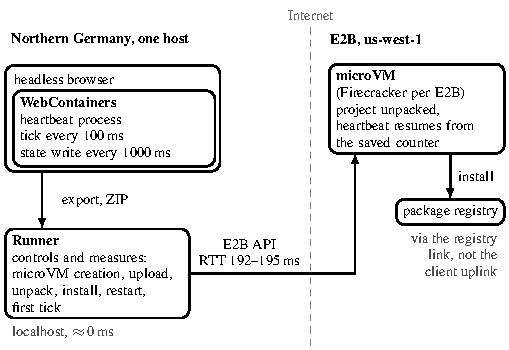
\includegraphics[width=\columnwidth]{figures/setup-diagram.pdf}
  \caption{Source, runner and target and their role in this setup.}
  \label{fig:setup}
\end{figure}

\subsection{Experimental design}

In the \textbf{size study}, two strategies are crossed with four project sizes, the size of the payload in the full copy. These four sizes are the levels small (\SI{1.8}{\kilo\byte}), light (\SI{0.91}{\mega\byte}), medium (\SI{4.62}{\mega\byte}) and large (\SI{13.93}{\mega\byte}). A cell is one strategy at one level. This gives eight cells at 30 repetitions and 240 runs. The script changes the order of the cells randomly within every cycle, in which each cell runs once. A handover can happen at any point between two state writes. Therefore, the script draws the stop offset, the time from the last state write to the stop, uniformly between 0 and \SI{1000}{\milli\second}. The order and the stop offsets come from a fixed seed, so the measurement session can be repeated.

\textbf{Manifest-based transfer} sends only the sources, the package manifest, the lockfile and the files of the heartbeat, \SIrange{1.7}{17.2}{\kilo\byte} in total.

The \textbf{live study}, named after live migration, is run on the large level only. The full copy transfers the most bytes at this level, so the push phase of pre-copy can move the most work before the stop. Two strategies with a push phase are added to the full copy and manifest-based transfer. At 30 repetitions each, this gives 120 runs, again with a fixed seed and a random order of the cells within every cycle. 
\textbf{Pre-copy} sends the full working directory to the target before the stop. 
\textbf{Manifest-push} sends it without the installed dependencies and runs the install on the target before the stop.

In every run, the browser page is reloaded, the WebContainers instance installs the dependencies of the level and the heartbeat starts. For the full copy and manifest-based transfer, the source stops the heartbeat at the drawn offset after three state writes. Afterwards, it exports the working directory and posts it to the runner. After the runner receives the archive, it creates a fresh microVM. Then it uploads and unpacks the archive and runs the install for manifest-based transfer. Lastly, it restarts the heartbeat from the exported state and waits for the first new tick. For pre-copy and manifest-push, the export, the microVM creation, the upload and the unpack take place before the stop. At the stop, only the files changed since the push follow, including the state file.

Each level carries at most one direct dependency with a fixed lockfile. The light level adds \texttt{express}, the medium level \texttt{@babel/preset-env} and the large level \texttt{aws-sdk}. These packages were chosen by their size and the duration of their install. The small level acts as a control without any dependency, so both strategies transfer about the same bytes. The light level installs 68 packages, the medium level 135 and the large level only 45.

\subsection{Dependent variables}

Four variables are recorded per run, and a fifth one for the strategies with a push phase. 
The \textbf{interruption time} runs from the stop on the source to the first tick on the target. It corresponds to the downtime in the migration literature \cite{clark2005live}. With a pull phase \cite{hines2009post}, it would only contain the files accessed before the first tick. After the restart, the heartbeat, whose first tick ends the interruption, accesses only three files. Hence, the interruption time of post-copy would hardly depend on the project size. Hybrid migration would fetch the files that pre-copy sends at the stop. Therefore, neither is measured, and the target needs no layer that fetches missing files on access.
With a push phase, the \textbf{total handover time} adds the push phase to the interruption time. Without a push phase, it equals the interruption time. It is split into the phases transfer, install, target start and harness. The target start consists of microVM creation, restart of the heartbeat and first tick. The transfer consists of export, upload and unpack. The harness is the overhead of the measurement setup.

The \textbf{bytes transferred} are the size of the archive which crosses the boundary. For the strategies with a push phase, this is the archive sent at the stop. The \textbf{state loss} is the number of ticks between the last state write and the stop, both read on the source after the stop. 
Lastly, the \textbf{source shortfall} compares the ticks of the source during the push phase with the ticks expected at its idle rate. The idle rate is the number of ticks per second the heartbeat reaches when the source does nothing else. It is measured as the increase of the state loss per second of stop offset over the 120 runs of the live study.

Each run is correct if the target loads the exported counter and keeps counting.

\subsection{Interruption time across two clocks}

The interruption time starts with a timestamp right before the stop on the source and ends with the first new line in the log of the heartbeat on the target. In all 360 runs, the clocks of the browser and the runner differ by $-0.5$ to \SI{+0.5}{\milli\second}, which is the resolution of the measurement. Therefore, only the clock of the target is converted to the clock of the runner. Its offset is estimated in every run with Cristian's method. The runner asks the target for its time and measures the round trip of this request. The target reads its clock at some point within this round trip, so the estimate is off by at most half of it \cite{cristian1989probabilistic}. The runner reads the clock five times and keeps the reading with the shortest round trip, without considering clock drift.

\subsection{Statistical treatment}
The interruption time and the state loss are reported as medians, the phases of the total handover time in Figure~\ref{fig:decomposition} as means. The dispatch of the restart command, from its call at the runner to its start on the target, is bimodal in all twelve cells. Therefore, medians, a bootstrap confidence interval and a permutation test are used, as none of them assumes a normal distribution. According to Papadopoulos et al., such data may need methods without this assumption, and bootstrap sampling can make the evaluation more robust \cite{papadopoulos2019methodological}.

RQ-2 is answered by a bootstrap confidence interval and a two-sided permutation test on the median difference between the strategies per level. Both use 10,000 draws and a fixed seed. The interval is the 2.5th to 97.5th percentile of the bootstrap distribution, and no correction is applied across the four levels. The crossing point is placed on a straight line between the two adjacent levels at which the median difference changes sign. Its interval comes from the same bootstrap draws. In both measurement sessions, the full copy and manifest-based transfer run at the large level. The intervals of their differences are too wide to show that the measurement sessions are the same. Therefore, cells are compared only within a study.

In the live study, the primary comparisons were fixed before the measurement session. These are pre-copy against the full copy and manifest-push against manifest-based transfer on the interruption time. They use the same bootstrap interval and permutation test. The comparison of pre-copy with manifest-push and every comparison of the total handover time are post hoc. Furthermore, no run is discarded.

\section{Results}
\label{sec:results}

In all 360 runs, the target loaded the exported counter and kept counting.

\subsection{Live study (RQ-1)}

The full copy and manifest-based transfer reach median interruption times of \SI{8.74}{\second} and \SI{6.91}{\second}. Pre-copy reaches an interruption time of \SI{1.69}{\second} and a total handover time of \SI{9.90}{\second}. For manifest-push, these values are \SI{1.57}{\second} and \SI{8.17}{\second}. At the stop, the full copy sends \SI{13.93}{\mega\byte} and manifest-based transfer \SI{7.45}{\kilo\byte}. Pre-copy and manifest-push only send \SI{1.16}{\kilo\byte} and \SI{1.15}{\kilo\byte} at the stop.

In the primary comparisons, pre-copy lowers the median interruption time by \SI{7.05}{\second} compared to the full copy (95\,\% CI \SIrange{6.52}{7.47}{\second}). For the full copy, the microVM creation has a median of \SI{0.84}{\second}. Manifest-push lowers the median interruption time by \SI{5.34}{\second} compared to manifest-based transfer (95\,\% CI \SIrange{5.01}{5.71}{\second}). For manifest-based transfer, the install and the microVM creation have medians of \SI{4.34}{\second} and \SI{0.93}{\second}. Both permutation tests give $p \leq 0.0001$.

Between pre-copy and manifest-push, the interruption time differs by \SI{119}{\milli\second} (95\,\% CI \SIrange{-95}{559}{\milli\second}). The interval includes zero. The source shortfall of pre-copy has a median of 14.5\,\%, with a range of 10.3 to 17.2\,\%. The source of manifest-push stays within 4\,\% of its idle rate.

In total, pre-copy takes more time than the full copy. The difference is \SI{1.16}{\second} (95\,\% CI \SIrange{0.55}{1.59}{\second}), and against manifest-push it is \SI{1.73}{\second} (95\,\% CI \SIrange{1.14}{2.40}{\second}).

\subsection{Size study (RQ-2)}

\begin{table}[t]
\caption{Interruption time of the size study in seconds, as median and \ac{IQR} over 30 runs per cell.}
\label{tab:interruption}
\centering
\scriptsize
\setlength{\tabcolsep}{3pt}
\begin{tabular*}{\columnwidth}{@{\extracolsep{\fill}}lrrrrr@{}}
\toprule
Level & Payload & Full & Manifest & \multicolumn{2}{c}{Full $-$ Manifest} \\
\cmidrule(l){5-6}
 & & median (\acs{IQR}) & median (\acs{IQR}) & median & 95\,\% CI \\
\midrule
small  & \SI{1.8}{\kilo\byte}   & 3.02 (0.51) & 3.12 (0.76) & $-0.10$ & $[-0.38, 0.27]$ \\
light  & \SI{0.91}{\mega\byte}  & 3.66 (0.80) & 5.72 (1.08) & $-2.05$ & $[-2.54, -1.55]$ \\
medium & \SI{4.62}{\mega\byte}  & 5.44 (0.53) & 7.39 (1.33) & $-1.95$ & $[-2.56, -1.52]$ \\
large  & \SI{13.93}{\mega\byte} & 8.71 (0.77) & 6.95 (0.96) & $+1.76$ & $[1.42, 2.21]$ \\
\bottomrule
\end{tabular*}
\end{table}

\begin{figure}[t]
  \centering
  \includegraphics[width=\columnwidth]{figures/decomposition.pdf}
  \caption{Mean of each phase of the total handover time in the size study, 30 runs per cell.}
  \label{fig:decomposition}
\end{figure}

Manifest-based transfer is slower than the full copy at the light and the medium level. At the large level it is faster (Table~\ref{tab:interruption}). At these three levels the permutation test gives $p \leq 0.0001$. At the small level the difference lies in an interval that includes zero ($p = 0.55$).

Therefore, the sign of the difference changes between the medium and the large level, from \SI{4.62}{\mega\byte} to \SI{13.93}{\mega\byte}. The estimated crossing point is \SI{9.5}{\mega\byte} (95\,\% CI \SIrange{8.7}{10.4}{\mega\byte}).

Figure~\ref{fig:decomposition} shows where the difference arises. The transfer of the full copy grows with the payload from \SI{1.26}{\second} at the small level to \SI{7.03}{\second} at the large one. For manifest-based transfer, it stays at \SIrange{1.32}{1.42}{\second} at every level. In return, manifest-based transfer runs the install on the target. This takes \SI{3.01}{\second} at the light level, \SI{4.88}{\second} at the medium and \SI{4.47}{\second} at the large one. The install is shorter than the saved transfer time only at the large level, where \SI{5.71}{\second} of transfer time are saved. At the medium level the saved transfer time is \SI{2.31}{\second} and at the light level \SI{0.75}{\second}. Additionally, at the three upper levels, the target start of manifest-based transfer is \SIrange{0.39}{0.46}{\second} shorter than for the full copy.

The state loss has a median of five ticks over all 240 runs and four to six ticks per cell.

\section{Discussion}
\label{sec:discussion}

If the handover is anticipated, the push phase moves most of the work to the time before the stop. For pre-copy this is the transfer, for manifest-push the install. As derived (RQ-1), the push phase shortens the interruption time in the live study. Part of this reduction comes from creating the target before the stop. However, pre-copy has a longer total handover time than the full copy. Both correspond to Clark et al., who reserve the resources on the target before the copy and describe how to balance the downtime against the total migration time \cite{clark2005live}. Furthermore, the push phase of pre-copy puts extra work on the source, which shows in its source shortfall (Section~\ref{sec:results}). For a source close to its limit, this speaks in favor of manifest-push.

A single push round is enough in this setup. In all 60 runs with a push phase, only three small files follow at the stop. Two of them, the log and the state file, form the small writable working set of the heartbeat (Section~\ref{sec:related-work}), which makes it an easy case for pre-copy \cite{clark2005live}. Further rounds wouldn't help with the heartbeat, because it keeps writing to its files, so the set of changed files doesn't shrink.

Without anticipation, the choice between the full copy and manifest-based transfer depends on the project size (RQ-2). At the large level, manifest-based transfer is faster mainly because it moves most of the transfer from the uplink of the client to the registry link of the target. Therefore, this advantage depends on the registry link, which isn't varied in this setup.

At the small level, both strategies still take about \SI{3}{\second} in the median (Table~\ref{tab:interruption}). This size-independent share of E2B in us-west-1 applies to strategies that create the target after the stop, so the interruption doesn't grow proportionally with the project size.

Part of this share is the network path to the US. A target closer to the client would shorten it. The shortest round trip to the target has a median of 192 to \SI{195}{\milli\second} in every cell. Within the interruption, the runner makes four calls to E2B one after another for the full copy, five for manifest-based transfer with an install and three for the push strategies. For comparison, gcping measured an HTTP latency of \SI{195}{\milli\second} from Northern Germany to Google Cloud us-west1, where the default region of E2B runs \cite{e2b-egress-2026}, and \SI{41}{\milli\second} to europe-west3 \cite{gcping-2026}.

\subsection{Threats to Validity}

The heartbeat neither loads nor writes its dependencies. Therefore, a successful install only means that the install command ends without an error. Furthermore, the dependencies never change on the source during the push phase, which both push strategies assume. The heartbeat counter is the only process state that crosses the boundary, because the heartbeat writes it to a file. Since there is no memory image, state such as open connections or the module graph of a development server would be lost at every handover. Lastly, the full copy and pre-copy send the dependencies installed in WebContainers unchanged to the target, and none of the three packages carries binaries for a specific platform.

Only one client is used, and each study runs in one measurement session with one uplink, one region and one hosted target. Furthermore, the load on the E2B hosts isn't under control. For manifest-based transfer, the bytes transferred only count the archive and not what the install downloads from the registry. The handover is triggered by the script, as the WebContainers \ac{API} documents no signal before a resource runs out \cite{stackblitz-2024}. Hence, detecting that a resource runs out isn't part of the interruption time.

Within this setup, the crossing point depends on four further factors. First, each upper level carries a different direct dependency. Hence, the effect of the size can't be separated from the effect of the packages. Second, every megabyte adds about \SI{242.8}{\milli\second} of upload time over the 120 runs of the full copy. If the uplink were half as fast, the crossing point would move to \SI{5.9}{\mega\byte}, and if it were twice as fast, to \SI{13.7}{\mega\byte}. Third, the phases on the client lie inside the interruption time. For the full copy at the large level, they take 16.3\,\% of the median interruption time, almost all of it for the export. For manifest-based transfer, they take less than 1\,\%. Therefore, a weaker client would move the crossing point towards smaller projects. Lastly, the straight line between the medium and the large level was chosen after the measurement session. Other estimates from the same data compare the transfer, the install and the target start instead of the interruption time. In these estimates, the transfer of the full copy grows with the payload on a straight line over its 120 runs. The install of manifest-based transfer is taken from one of the three upper levels. Depending on this level, the crossing point lies between 5.8 and \SI{10.3}{\mega\byte}.

A Bonferroni correction across the four levels raises the bound of $p$ to 0.0004 and changes none of the results. The interruption time also depends on reading the clock of the target (Section~\ref{sec:methodology}). The bound of the reading error, half of the shortest round trip of each run, is at most \SI{337}{\milli\second}. Therefore, the difference between two strategies changes by at most \SI{674}{\milli\second}, which is smaller than the differences at the three upper levels and in the primary comparisons.

\section{Conclusion and Future Work}
\label{sec:conclusion}

Without a memory image, three parts of migration theory still apply, the split into cold and live migration, the downtime and the total migration time. However, the strategies have to transfer files instead of memory pages. All four migration types of He and Buyya have a counterpart at the filesystem level, each with its own condition (RQ-1). Pre-copy requires an anticipated handover, and post-copy needs the browser tab to stay open until the pull phase ends. Hybrid migration depends on both of these conditions. Pre-copy and cold migration are the two types measured in this work. In the live study at the large level, both push strategies create the target before the stop and use a single push round. This lowers the median interruption time of the heartbeat from \SI{8.74}{\second} to \SI{1.69}{\second} for pre-copy and from \SI{6.91}{\second} to \SI{1.57}{\second} for manifest-push. However, pre-copy takes longer than the full copy in total. Without anticipation, manifest-based transfer beats the full copy from a project size between the medium and the large level (RQ-2). For these four projects on E2B, this size lies between \SI{4.62}{\mega\byte} and \SI{13.93}{\mega\byte}. It may also depend on their packages, on the uplink of the client and on the registry link of the target.

In future work, the handover could be compared with a cooperative case, in which the runtime can be controlled and the memory can come along. With such a comparison, the cost of the missing memory image could be measured. How much the choice of source and target affects the results could be measured with other sources and targets. Furthermore, post-copy and hybrid migration could be measured after the first tick with a workload that reads its files. Additionally, it could be measured whether and how often a session reaches the limits of the sandbox in practice and whether the source can observe this in advance.

\section*{Acknowledgment}

\textbf{Use of generative AI.} The authors used generative AI tools (Claude Code with Claude Opus 5 and 5.5 by Anthropic, Google NotebookLM and Gemini 3.5) as assistants, under their own direction and review: for structuring and literature search, for drafting and editing sections, which the authors revised, and for implementing and testing the measurement setup, analysis script, and figure code. All measurements were carried out by the authors on the infrastructure described in Section~\ref{sec:methodology}. All measured data and results are derived from these experiments, and every cited source was checked against the original publication. The authors take full responsibility for the entire content and narrative of this paper.


\newrefcontext
\printbibliography

\end{document}
